
\rhead{Enclosure Escape}

\chapter{Enclosure Escape}
\label{sec:enclosure_escape}

\begin{figure}[!h]
\centering
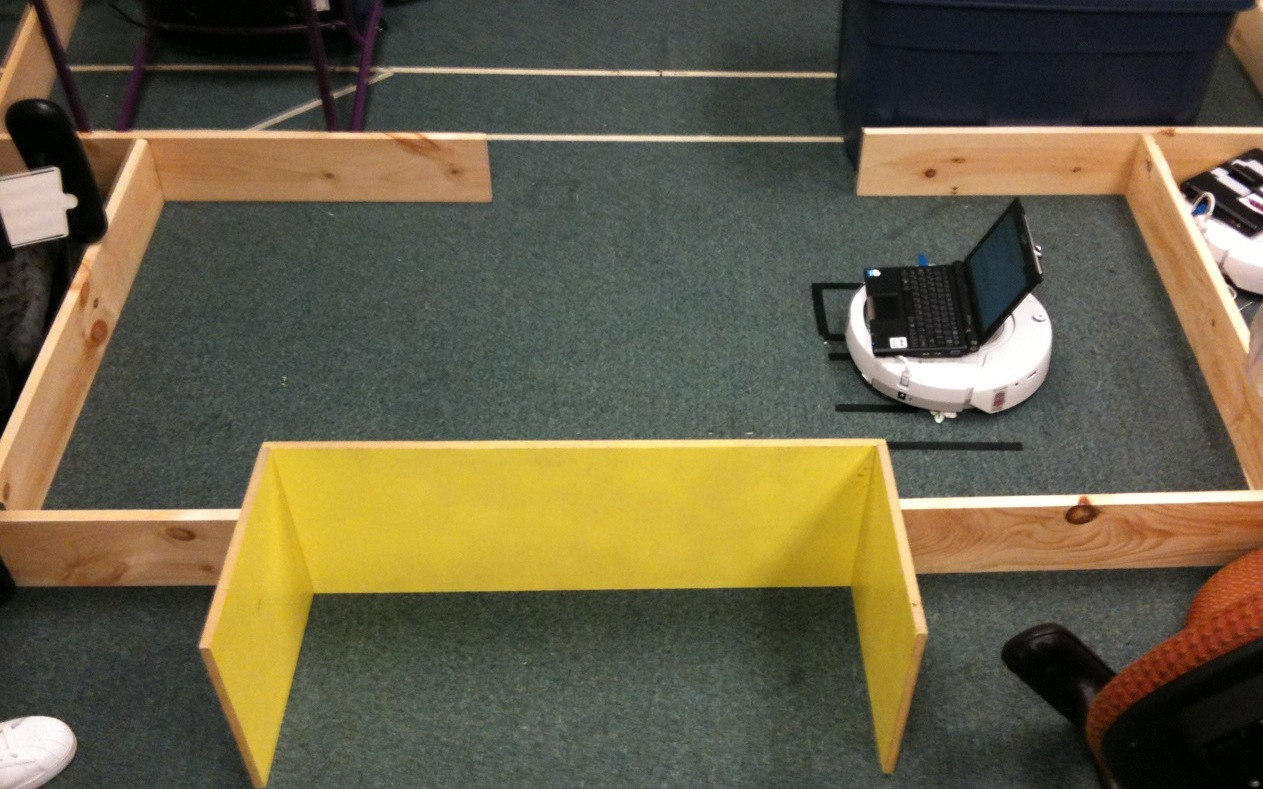
\includegraphics[width=1.0\columnwidth]{figures/5_teaser.jpg}
\end{figure}

\newpage

\section{Introduction}

The Enclosure Escape project is structured to acquaint students with the basics of writing robot clients that control basic planar movement using either Player/Stage/Gazebo (PSG) robot interface suite or \href{http://www.ros.org/wiki/ROS/StartGuide}{ROS (the Robot Operating System)}, which are the two middleware systems supported by our course staff. The students are tasked with implementing either a reactive or deliberative robot control policy to escape from an arbitrary static enclosure.

\vspace{5 mm}

\noindent At the end of this chapter you will...
\begin{itemize}
\item have basic knowledge of:

\begin{itemize}
% \item The Player or ROS robot middleware systems to write a client application.% this should go in chapter 3 instead
\item Deliberative and reactive robot control architectures.
\end{itemize}

\item be able to:

\begin{itemize}
\item Send commands to the robot to control its position.
\item Receive sensory information from the robot, specifically the bumper sensor.
\item Implement a deliberative control policy using random motion to allow the robot to escape from an enclosure.
\item Implement a reactive control policy using a Bug Algorithm to allow the robot to escape from an enclosure.
\end{itemize}

\end{itemize}

\section{Key Concepts}

\begin{figure}[!h]
\centering
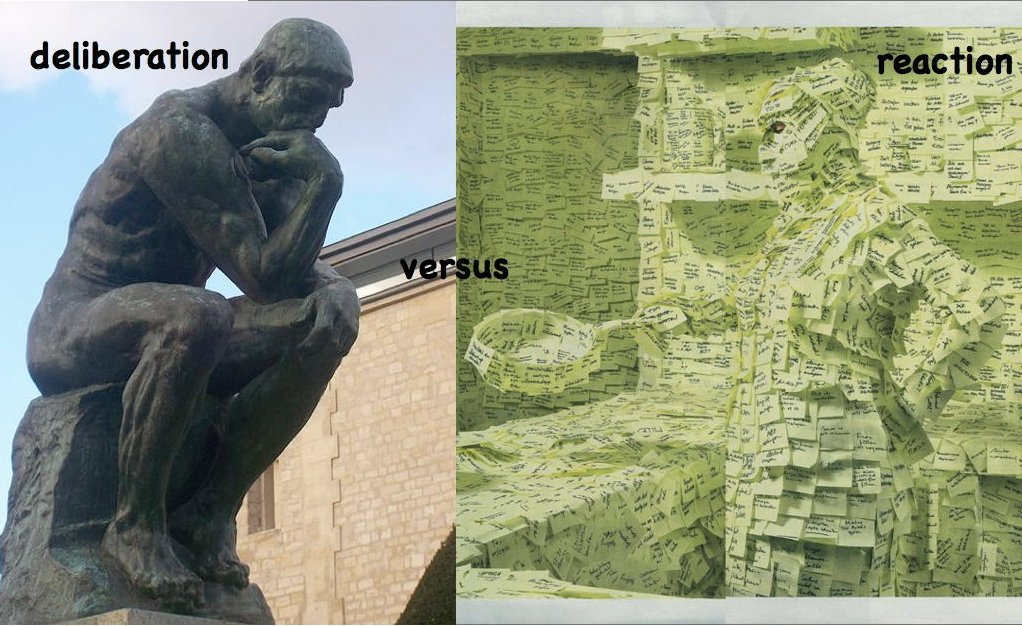
\includegraphics[width=0.6\textwidth]{figures/5_spectrum2.jpg}
\end{figure}


What approaches can we use to structure the robot control policy?\\

\noindent This project focuses on the Decision Making aspect (Figure \ref{fig:5_decision_making}) of the Robot Control Loop presented in Figure \ref{fig:1_control_loop}. For this project, the Perception component of the loop is enacted by the Player \href{http://playerstage.sourceforge.net/doc/Player-2.1.0/player/group\_\_playerc\_\_proxy\_\_bumper.html}{bumper} proxy. The Motion Control component of the loop is enacted by the Player \href{http://playerstage.sourceforge.net/doc/Player-2.1.0/player/group\_\_playerc\_\_proxy\_\_position2d.html}{position2d} proxy. The project focuses on the Decision Making component in which different approachs to autonomous control architectures can be employed. All control policies will react to a bumper, yet the various approachs to Decision Making differ in \emph{how} the robot will react to the bumper sensor.

\begin{figure}[!h]
\centering
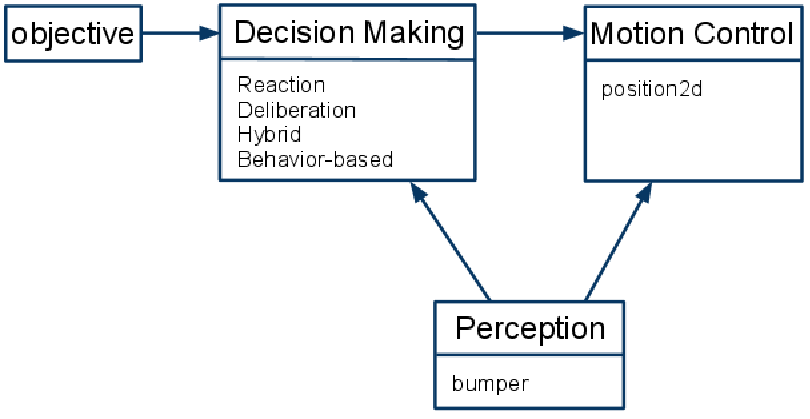
\includegraphics[width=0.5\textwidth]{figures/5_decision_making.png}
\caption{Approaches to the Enclosure Escape task cast within the Robot Control Loop.}
\label{fig:5_decision_making}
\end{figure}

\subsection{Reaction-Deliberation Control Policy Spectrum}

\begin{figure}[!h]
\centering
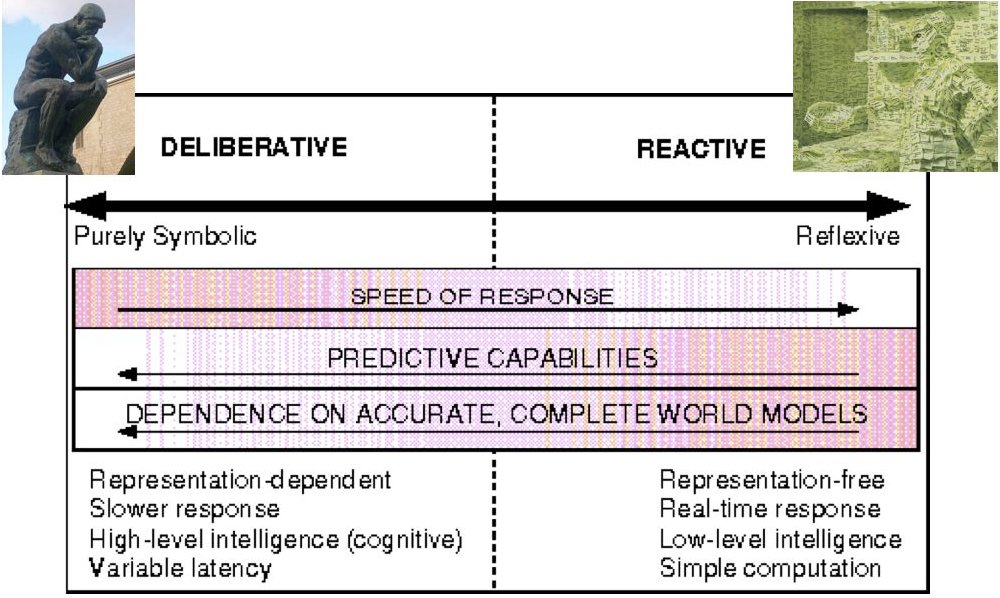
\includegraphics[width=0.85\textwidth]{figures/5_spectrum1.jpg}
\caption{Deliberation-Reaction spectrum. (Source unknown)}
\label{fig:5_spectrum}
\end{figure}

For the problem of esacping an enclosure, different control architectures can be used for decision making that range from deliberative control to reactive control, including a combination of both approaches that lie along the spectrum presented in Figure \ref{fig:5_spectrum}. If a purely reactive policy is used, the robot simply reacts, making a decision based only on the most recent bumper information perceived in its current iteration of the control loop. A reactive policy does not store history information and is not concerned with what will happen in the future. If a deliberative policy is used we try to build a larger understanding of the world state based on a history of bumper information and a future outlook on what the robot should do. A deliberative system has a purely high level symbolic or probabilistic representation of all possible decisions. 

There are many tradeoffs between a deliberative and a reactive system, the first tradeoff being speed. A reactive system is very fast since it only makes a decision based on a hard-coded rule, for the current time step. A deliberative system will be slower since it searches over all, or many, possible outcomes. If planning takes too long, the performance of the system will suffer and the robot will not be able to respond in a highly dynamic environment. Secondly, to be able to consider all possible decisions, deliberation has a dependecy on a complete world map, requiring the state estimation to be accurate and the perception system to be, ideally, noise-free. Since a reactive policy only reacts, it does not need a representation of the world and an accurate estimation of the perceived state is not as critical. Thus a reactive system is beneficial if a robot application needs to be fast, simple amd does not require a lot of memory to store world models. However the application is best at performing one specific task and a downfall of such a system is it will make the same mistakes over and over. A deliberative system is beneficial for tasks that require a higher level of intelligence, however it will be slower, requires an accurate world representation and it is crucial that the system can update the world state fast enough so the representation is not out-of-date or inaccurate. 

\subsubsection{Types of Robot Policies}\footnote{cite ``The Robotics Primer"}

\begin{itemize}
\item Deliberative Control: ``Think hard, act later."

\begin{figure}[!h]
\centering
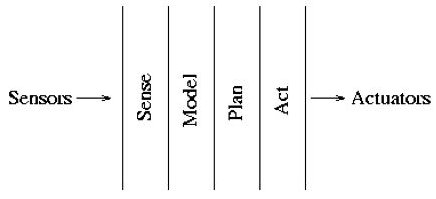
\includegraphics[width=0.5\textwidth]{figures/5_deliberation.jpg}
\caption{Delibartion. (Source unknown)}
\label{fig:5_deliberation}
\end{figure}

Deliberative, or Planner-based control employs a Sense-Plan-Act paradigm, as seen in Figure \ref{fig:5_deliberation}. First the robot senses based on the sensory information it receives and builds a most complete model of the world using the perceived information. Second the robot plans by searching over all, or a subset of all possible outcomes. Third the robot acts by executing a plan through motor forces and sending commands to the actuators. These three steps are continually executed in a serial fashion. 

\begin{figure}[!h]
\centerline{
\mbox{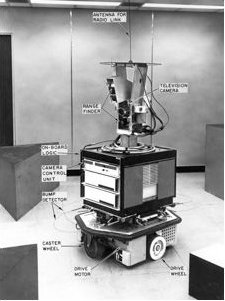
\includegraphics[width=1.0in]{figures/5_shakey.jpg}}
\mbox{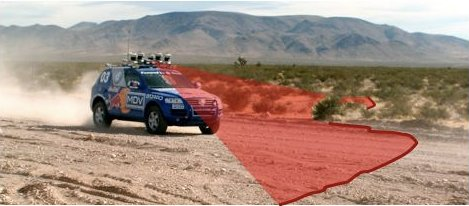
\includegraphics[width=2.0in]{figures/5_stanley.jpg}}
\mbox{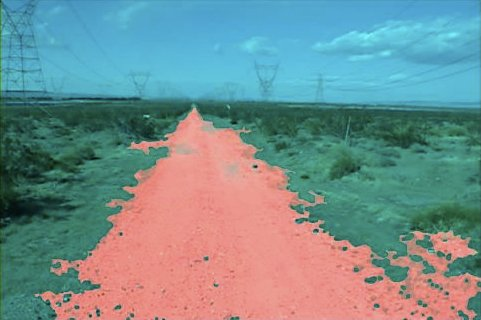
\includegraphics[width=2.0in]{figures/5_path.jpg}}
}
\caption{Deliberative control robotic applications: Shakey of SRI; Stanford's Stanley Robot Car in the DARPA Grand Challenge.}
\label{fig:5_shakey_stanley}
\end{figure}

Deliberative systems are best at applications that require thinking hard and where looking ahead is essential for making decisions. Example algorithms in which thinking hard is appropriate for finding a solution include Breadth First Search, Depth First Search, Dijkstra's Algorithm or A* Search. Example robotic applications include Shakey the Robot and navigating the DARPA Grand Challenge, as seen in Figure \ref{fig:5_shakey_stanley}.

% - sense-plan-act paradigm
% - sense: build most complete model of world
% - plan: search over all possible outcomes
% - act: execute plan through motor forces
% - example algorithms: BFS, DFS, Dijkstra, A*
% - example robotic applications: Shakey, Grand Challenge

\item Reactive Control: ``Don't think, (re)act."

\begin{figure}[!h]
\centering
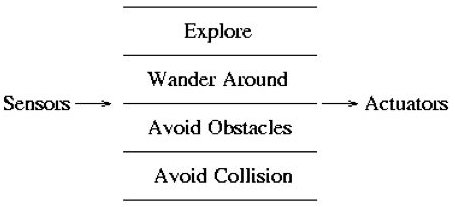
\includegraphics[width=0.5\textwidth]{figures/5_reaction.jpg}
\caption{Reaction. (Source unknown)}
\label{fig:5_reaction}
\end{figure}

Reactive control policies have no representation of state and they do no search over possible outcomes to make a decision. Instead, as seen in Figure \ref{fig:5_reaction}, reactive control is based on a set of modules implemented as hardcoded rules that map sensory inputs to actuator outputs. More specifically, there exists a set of conditions that are either true or false based on what is currently sensed and a set of actions that each condition specifies. A reactive system is typically very fast since the system does not think, it simply reacts. A subsumption architecture, which is studied in Chapter \ref{sec:subsumption}, is a reactive system consisting of prioritized rules or reactive policies. Each rule achieves a desired task, such as avoid-obstacle or go-to-ball, and the entire collection of prioritized modules aims to achieve a larger goal, such as playing robot soccer.

Reactive control encompasses the notion of embodied intelligence, in which the intelligence of a system (or the ability of a system to perform a specific task) is achieved through interaction with the environment driven by perception and action and not a prespecified algorithm. The overall behavior of the system is not based on planning or explicit decision making algorithms, but rather the interaction of the control policy and embodiment with the environment. An example of embodied intelligence is ant stigmergy in which ants leave pheromone trails to communication with each other. Ants lay pheromones on their way back to the nest after they have found food; new ants that emerge from the nest simply follow the pheronomes to find food. Leaving trails in such a way produces a complex network of trails and efficiently connects the nest to different food sources\footnote{http://en.wikipedia.org/wiki/Stigmergy}. Thus ants can produce what looks like intelligent behavior, although they are only capable of very simple cognitive skills. The intelligent behavior emerges based on ants using a simple control policy driven by perception and action while interacting with the given environment.

\begin{figure}[!h]
\centerline{
\mbox{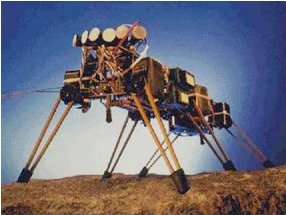
\includegraphics[width=2.0in]{figures/5_ant.jpg}}
\mbox{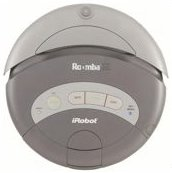
\includegraphics[width=1.5in]{figures/5_roomba.jpg}}
\mbox{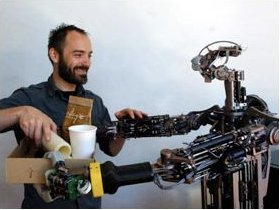
\includegraphics[width=2.0in]{figures/5_humanoid.jpg}}
}
\caption{Reactive control robotic applications.}
\label{fig:5_reactive_apps}
\end{figure}

Figure \ref{fig:5_reactive_apps} shows different reactive control robotic applications, including the Roomba which is at the heart of a reactive system. 

% - No representation of state
% - Typically, fast hardcoded rules
% - Embodied intelligence (1) behavior $\leftarrow$ control + embodiment (2) ant analogy, stigmergy
% - Subsumption architecture - prioritized reactive policies

\item Hybrid Control: ``Think and act separately \& concurrently."

\begin{figure}[!h]
\centering
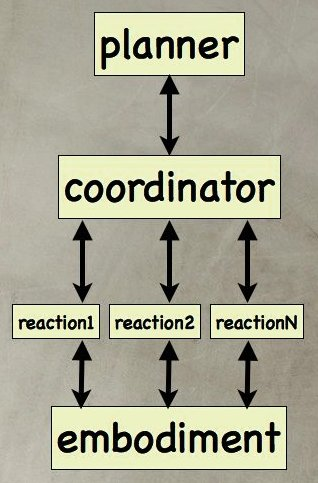
\includegraphics[height=0.4\textwidth]{figures/5_hybrid.jpg}
\caption{Hybrid System.}
\label{fig:5_hybrid}
\end{figure}

A hybrid system is top-down planning and low-level reaction. It combines both deliberative and reactive control, drawing upon the advantages of each: brains and speed respectively. As in Figure \ref{fig:5_hybrid}, at the top layer of a hybrid system is a top-down planner in charge of high-level or long term goals. At the bottom is a reactive layer that receives sensory information from and sends actuator commands to the embodiment. In between the two layers is a coordination layer that serves as an interface between the planner and the reaction modules. The coordinator is the meat of a hybrid system yet it poses a real challenge. While allowing the two layers to communicate, it must balance between long and short term goals, handle differences in representation of state and resolve conflicts between the deliberative and reactive components of the system.\footnote{``The Robotics Primer" p. 177-178.}

% - Top-down planner for high-level goals
% - Reaction for low-level immediate execution
% - Interface layer to coordinate - how to balance long and short term
% - modern cost maps?
% - Not discrete-continuous hybrid control

\item Behavior-Based Control: ``Think the way you act."

Behavior-based systems stem from a reactive control model and are an alternative approach to hybrid control. Instead of a top-down hierarchy consisting of two layers that separately implement planning and reaction, behavior-based control contains a set of modules or ``behaviors", each with equal priority. Each module has access to sensing and outputs motor commands. This model may seem similar to reactive control, however the difference is that the modules of reactive control can only enact simple actions such as ``reverse if both bumper sensors are pressed". A reactive system's modules are relatively simple because they can only react based on what is sensed in the current time instace. However a behavior-based system's modules can keep a history of sensory information, maintain state variables and send information between modules. Thus these modules can enact more complex behaviors such as ``avoid obstacle while obstacle in view". Individual modules maintain goals and can be either deliberative, reactive, or a combination of both. Modules handle both planning and reaction, as opposed to a hybrid system that has a single planner.

\begin{figure}[!h]
\centerline{
\mbox{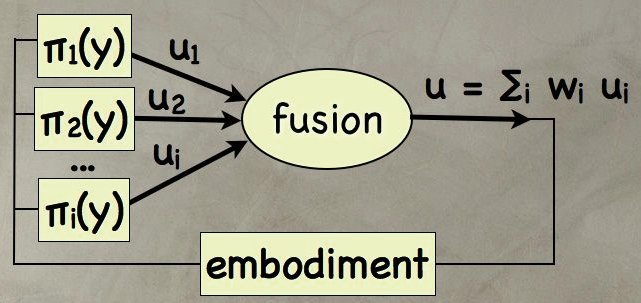
\includegraphics[height=1.5in]{figures/5_fusion.jpg}}
\mbox{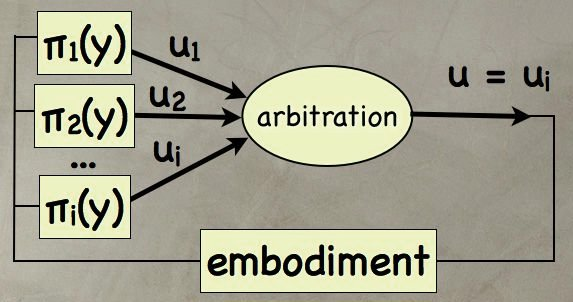
\includegraphics[height=1.5in]{figures/5_arbitration.jpg}}
}
\caption{Fusion (linearly combine) vs. Arbitration (winner-take-all)}
\end{figure}

% - All modules have equal priority, access to sensing, and output motor commands
% - Modules can be deliberative, reactive, or whatever
% - Commands merged through arbitration or fusion
% - potential fields?

% behavior based systems are another appraoch to doing this. instead of having a top down hierarchy have a bunch of modules all of which have equal priority. all these take in sensing information and output motor commands. these modules can be deliberative, reactive, whatever, as long as take in sensing info and output control command. these commands that are generated by all these systems are merged through arbitration process. if have fusion system find weights, find linear combination such that take weighted average of commands and thats the actual command i send to the robot. if have arbitration system, bunch of policies are sending me commands and i take the best one. winner take all.

\end{itemize}

\subsection{Policy Approaches for Enclosure Escape}

The navigation problem for Enclosure Escape is how to get from point A to point B. 

\subsubsection{Reactive: Random Traversal}

The simplest decision making policy to perform navigation is to employ a {\bf random walk}. For this assignment, a random walk is a good solution to this problem because eventually the robot will in fact navigate out of the enclosure. Specficially, random walk works well in terms of enclosed environments due to the notion of embodied intelligence. 

\vspace{5 mm}
\noindent The control policy can be implemented as follows: 
\begin{itemize}
\item If the bumper is not pressed: drive the the robot straight forward.
\item If the bumper is pressed: rotate the robot by a random amount.
\end{itemize}

\subsubsection{Deliberative: Bug Algorithm}

\begin{figure}[!h]
\centering
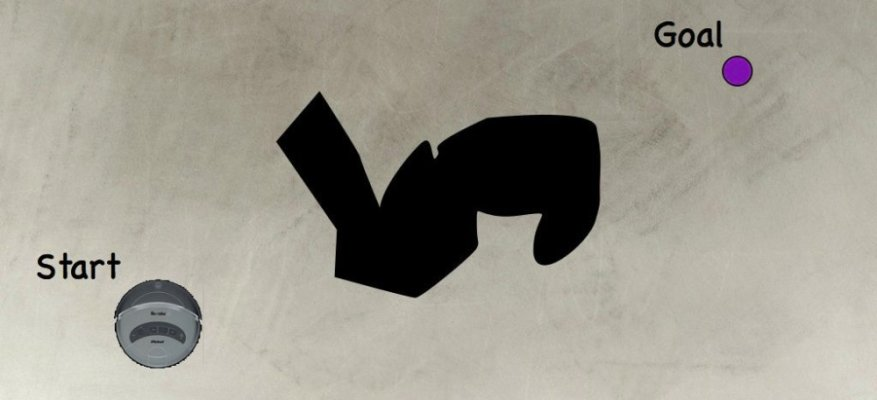
\includegraphics[width=0.75\textwidth]{figures/5_bug1.jpg}
\caption{Start of Bug Algorithm.}
\label{fig:5_bug1}
\end{figure}

\begin{figure}[!h]
\centering
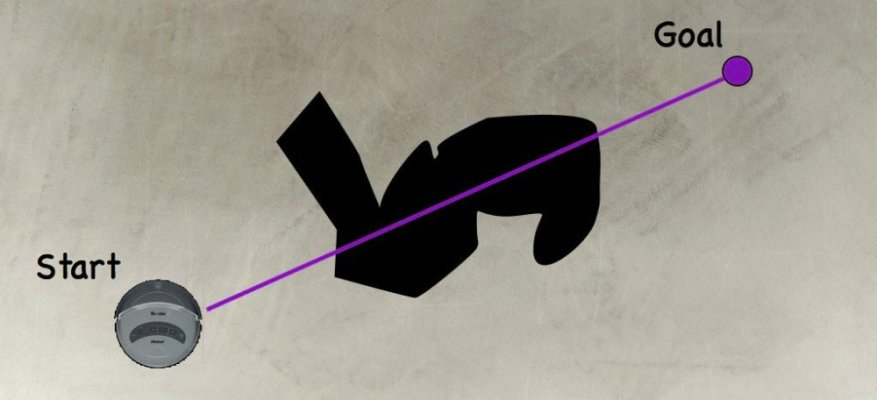
\includegraphics[width=0.75\textwidth]{figures/5_bug2.jpg}
\caption{Draw a straight-line path to the goal.}
\end{figure}

\begin{figure}[!h]
\centering
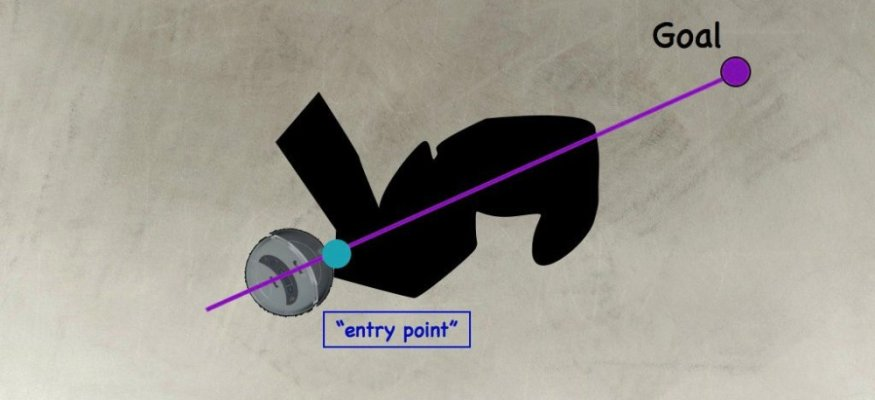
\includegraphics[width=0.75\textwidth]{figures/5_bug3.jpg}
\caption{Follow line until contact.}
\end{figure}

\begin{figure}[!h]
\centering
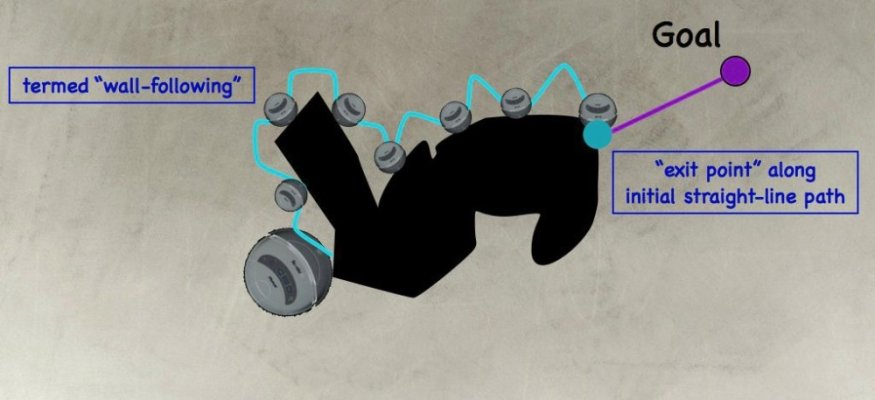
\includegraphics[width=0.75\textwidth]{figures/5_bug4.jpg}
\caption{Follow boundary around obstacle.}
\end{figure}

\begin{figure}[!h]
\centering
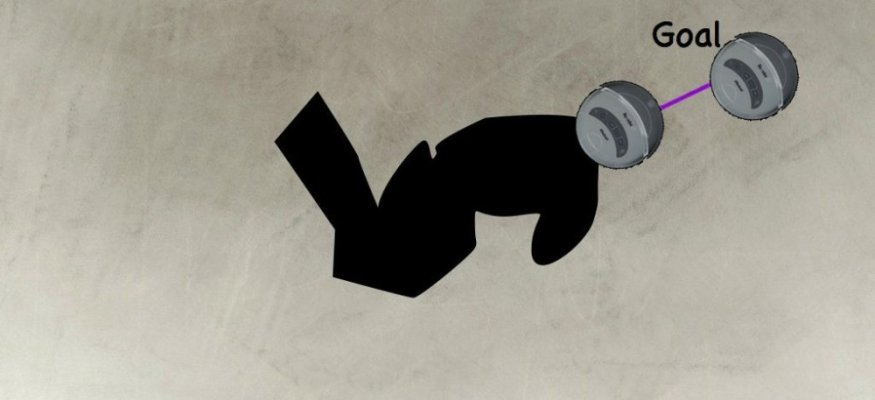
\includegraphics[width=0.75\textwidth]{figures/5_bug5.jpg}
\caption{Continue along straight-line path.}
\label{fig:5_bug5}
\end{figure}

The {\bf Bug Algorithm}\footnote{``Principles of Robot Motion: Theory, Algorithms, and Implementations"} is a ``simple" deliberative policy. The approach not only assumes bumper sensor information, but also localization or goal recognition. The Bug Algorithm is outlined in Figures \ref{fig:5_bug1} to \ref{fig:5_bug5}.

For this assignment, the Bug Algorithm may not be suitable since we are only using the bumper sensors which do not provide a capability to localize a goal location or recognize the enclosure opening. A modified version of the Bug Algorithm in the form of wall following can be employed for this assignment, however some randomness must still be introduced into the control policy to ensure escape. If the robot continually follows the interior wall, the robot will never escape the enclosure. We can add a timer to randomize the robot's turn direction after some period of time has elapsed, this will give the robot a chance to follow a different wall which will in turn allow the robot to escape.

\section{Project Infrastructure}

For this project, the iRobot Create platform comprising of the Create base and the ASUS EeePC subnotebook must be assembled, as described in \ref{sec:assembling_the_robot_platform}. Additionally, depending on which middleware framework is used, either Player or ROS must be installed on the EeePC, as described in Sections \ref{sec:player213} and \ref{sec:ros}, respectively.
 
Given this setup, both the Player server/ROS Master node and the robot client must run locally on the robot platform. However if a wireless network is available and the EeePC is connected to the network, then the robot client can also run on any computer that has Player or ROS installed. This is particularly helpful for development and debugging. The instructions below assume a locally running client.
 
\section{Instructions}

For this assignment, students are expected to work with either installation of Player or ROS on the EeePC to write a simple random traversal controller that reacts to obstacles using bumper sensing. Before writing your own controller, it is helpful to run through the instructions for sending commands to the robot and receiving sensory information using either Player or ROS, as described in Sections \ref{sec:player_quickstart} and \ref{sec:ros_quickstart}, respectively.

The second half of this project is to create a written report documenting the work done for this assignment. Specifically, students should run a number of experiments to evaluate how well the robot esacped from an enclosed area and how effective the implemented algorithm is. Students are encouraged to experiment with various enclosure escape algorithms and evaluate the relative performance of each. The details of how this report is graded are discussed in the following section.

\subsection{Player}

Note, these instructions are similar to those in Section \ref{sec:player_quickstart}.

\begin{itemize}

\item Start with the sample code provided in Section \ref{sec:player_quickstart} step \ref{sec:3_create_client}. This client simply rotates the robot in place and outputs the current bumper information to standard output, until Ctrl-c is pressed. 

\item Copy the below text to a file named \texttt{CMakeLists.txt}. This file uses the cmake build system to generate a Makefile for your program, as described in Section \ref{sec:3_cmake}. This file should reside in the same directory as \texttt{client.cpp}

\item Build a Makefile: \texttt{cmake .}

\item Compile the program: \texttt{make}

\item Copy the Player configuration file, \texttt{create.cfg}, from Section \ref{sec:player_quickstart} step \ref{sec:3_config_file}; it should reside in the same directory as \texttt{client.cpp}

\item Start the Player server: \texttt{player create.cfg}

\item Start the client: \texttt{./client localhost}\\
If running remotely: \texttt{./client <robot IP>}

\item Use the starter code to write a client to enable a SmURV robot to escape from an enclosure using a control policy discussed in this chapter.

\end{itemize}

\subsection{ROS}

\begin{itemize}

\item From the ROS root directory on the EeePC: \texttt{cd ros-1.0.0/pkg}\\
(Don't forget to \texttt{source rosenv} from the ROS root directory).

\item Create a ROS package for our controller:\\
\texttt{roscreate-pkg irobot\_create\_controller roscpp std\_msgs irobot\_create\_2\_1}\\
The \texttt{roscreate-pkg} command-line tool automatically creates a new ROS package called \texttt{irobot\_create\_controller} with dependencies on three other packages (\texttt{roscpp}, \texttt{std\_msgs} and \texttt{irobot\_create\_2\_1}). It generates a number of files for building the new package.

\item Create a \texttt{client.cpp} file in \texttt{irobot\_create\_controller/src} and add the following code to \texttt{client.cpp}:

\begin{verbatim}
#include <ros/ros.h>
#include <irobot_create_2_1/SensorPacket.h>
#include <geometry_msgs/Twist.h>
#include <signal.h>

ros::Publisher create_pub;
ros::Subscriber create_sub;

// Declare Ctrl-C related variables
bool endnow = false;
void stopper(int x)
{
  endnow = true;
}

// Master node calls this function everytime a new message arrives
void createListen(const irobot_create_2_1::SensorPacketConstPtr& msg)
{
  printf("Left: %d, Right: %d\n", msg->bumpLeft, msg->bumpRight);  
}

int main(int argc, char** argv) {

  // Initialize ROS
  ros::init(argc, argv, "controller");
  // Create a handle to this process node
  ros::NodeHandle n;
  // Publish messages of type geometry_msgs/Twist on topic "cmd_vel"
  create_pub = n.advertise<geometry_msgs::Twist>("cmd_vel", 1);
  // Subscribe to the "sensorPacket" topic.
  create_sub = n.subscribe("sensorPacket", 0, createListen);

  // Tell the function 'stopper' to receive all SIGINT signals	
  signal(SIGINT,stopper);

  while(!endnow)
    {
      double forward = 0.0;
      double rotate = 0.3;

      // Create and publish a Twist message
      geometry_msgs::Twist twist;
      twist.linear.x = forward; twist.linear.y = 0; twist.linear.z = 0;
      twist.angular.x = 0; twist.angular.y = 0; twist.angular.z = rotate;
      create_pub.publish(twist);

      ros::spinOnce();
    }

  // Stop the robot's movement
  geometry_msgs::Twist twist;
  twist.linear.x = 0; twist.linear.y = 0; twist.linear.z = 0;
  twist.angular.x = 0; twist.angular.y = 0; twist.angular.z = 0;
  create_pub.publish(twist);

  printf("Done.\n");
	
  return(0);
}
\end{verbatim}

The Create driver publishes a single message type, \texttt{SensorPacket.msg}, which exports all of the robot's sensory information. The message file exists in:\\ ros-1.0.0/pkg/irobot\_create\_2\_1/msg/SensorPacket.msg\\ 
For online documentation, visit the Brown ROS Create Driver \href{http://code.google.com/p/brown-ros-pkg/wiki/irobot\_create\_2\_1}{site}.

Additionally, use this \href{http://www.ros.org/wiki/ROS/Tutorials/WritingPublisherSubscriber(c\%2B\%2B)}{ROS tutorial} as a helpful resource for writing simple Publish and Subscriber nodes in C++.

\item Edit \texttt{irobot\_create\_controller/CMakeLists.txt} and add the following line to the end of the file:\\
\texttt{rosbuild add executable(client src/client.cpp)}\\
This causes an executable named \texttt{client} to be created whenever you run the command \texttt{rosmake irobot\_create\_controller}. For more information on CMake, refer to Section \ref{sec:3_cmake}, however most of the work in creating CMakeLists is done automatically by ROS.

\item Compile: \texttt{rosmake irobot\_create\_controller}

\item Turn on the Create base and the EeePC.

\item Run the ROS master: \texttt{roscore}

\item Run the Create driver: \texttt{rosrun irobot\_create\_2\_1 driver.py}

\item Run the controller client: \texttt{rosrun irobot\_create\_controller client}

\end{itemize}
 
\section{Expected Outcomes and Reports}

The following outlines our grading criteria:

\vspace{1cm}
\begin{tabular}{|l|l||l|l|}
\hline
{\large \bf Project Implementation} & \\
\hline
\hline
Movement Control & 20\% \\
$\rightarrow$ Does your robot move smoothly in the environment? & \\
\hline
Obstacle Reaction & 20\% \\
$\rightarrow$ Does your robot reasonably detect and respond to obstacles? & \\
\hline
Controller Robustness & 10\% \\
$\rightarrow$ Does your controller run without interruption? & \\
\hline
\end{tabular}

\section{Sample Client Code}

The starter code we give students in this assignment is the same code in Section \ref{sec:player_quickstart} using Player and section \ref{sec:ros_quickstart} using ROS.

\section{Solution Client Code using Player and ROS}: private svn link

\newpage

